\setcounter{page}{2}
\section*{Цели работы.}
Ознакомление с основными правилами формирования выборки и подготовки выборочных данных к статистическому анализу.

\section*{Постановка задачи.}
Осуществить формирование репрезентативной выборки заданного объема из имеющейся генеральной
совокупности экспериментальных данных.
Осуществить последовательное преобразование полученной выборки в ранжированный,
вариационный и интервальный ряды.
Применительно к интервальному ряду построить и отобразить графически полигон,
гистограмму и эмпирическую функцию распределения для абсолютных и относительных частот.
Полученные результаты содержательно проинтерпретировать.

\section*{Порядок выполнения работы.}
\begin{enumerate}
    \item Выбрать программное обеспечение или язык программирования и обосновать его выбор.
    \item Выбрать двумерную генеральную совокупность, предварительно согласовав её с преподавателем. Указать, откуда была взята генеральная совокупность и предоставить ссылку.
    \item Из генеральной совокупности сформировать выборку заданного объёма в соответствии с полученным от преподавателя номером. Указать, каким образом была сформирована выборка и какого вида она получилась.
    \item Последовательно преобразовать выборку в ранжированный, вариационный и интервальный ряды. Результаты содержательно проинтерпретировать и сделать выводы.
    \item Для интервального ряда абсолютных частот построить и отобразить графически полигон, гистограмму и эмпирическую функцию. Сделать выводы.
    \item Аналогичные действия выполнить для интервального ряда относительных частот. Сравнить результаты и сделать выводы.
\end{enumerate}

\section*{Основные теоретические положения.}
\textit{Генеральная совокупность} -- это совокупность всех объектов или наблюдений, относительно которых исследователь намерен делать выводы при решении конкретной задачи. В ее состав включаются все объекты, которые подлежат изучению.

\textit{Выборка} или \textit{выборочная совокупность} -- часть генеральной совокупности элементов, которая охватывается экспериментом.

\textit{Репрезентативность} выборки описывает способность выборочных данных отражать структурные свойства совокупности, из которой они были извлечены. Т.е. даёт ответ на вопрос: можно ли в исследовании заменить совокупность на выборку без значимого ухудшения результатов анализа.
Выделяют качественную и количественную репрезентативность.
Для оценки репрезентативности выборки могут быть использованы как статистические,
так и не статистические методы.

\textit{Вариационный ряд} -- это набор значений признака и их частот.
\textit{Ранжированный ряд} -- это упорядоченные (по возрастанию или убыванию) значения признака.
\textit{Интервальный ряд} -- это совокупность интервалов изучаемого признака, числа измерений, попадающих в выбранный интервал и/или
частот попадающих значений относительно объема выборки.

\textit{Полигон ряда частот} представляет собой линию, состоящую из точек $(x_i, f_i)$,
где $x_i$ -- значение середины $i$-того интервала, $f_i$ -- соответствующая частота.

\textit{Гистограмма частот} -- графическое представление распределения частот исследуемого
признака, образуемое соприкасающимися прямоугольниками, основаниями которых служат интервалы классов, а площади пропорциональны частотам этих классов.
Более формально, пусть $X_1, \dots, X_n$ - выборка, имеем разбиение $-\infty < a_0 < a_1 < \cdots < a_{k-1} < a_k < \infty$,
\begin{gather*}
    n_i = \sum_{j=1}^n \mathds{1}_{\{X_j \in (a_{i-1}, a_i]\}}, i = 1, \dots, k
\end{gather*}
тогда
\begin{gather*}
    h(x) = \frac{n_i}{n\Delta a_i}, \Delta a_i = a_i - a_{i-1}, i = 1, \dots k
\end{gather*}
называется нормализованной гистограммой.

\textit{Эмпирической функцией распределения} называется функция равная:
\begin{gather*}
    F_n(x) = \frac{1}{n} \sum_{i=1}^n \mathds{1}_{\{x_i < x\}}
\end{gather*}
Эмпирическую функцию можно также строить по интервалам.

\section*{Выполнение работы.}
Для выполнения работы был выбран язык Python3 и среда Jupyter Notebook с сервисом
Google Colab.

В качестве двумерной генеральной совокупности был выбран средний рост в сантиметрах
мужчин и женщин по странам мира.
Датасет был предоставлен пользователем Majyhain на сайте \textit{\href{kaggle.com}{kaggle.com}}.
Из датасета были отобраны первые 110 строк (110 стран, в которых в среднем самые высокие мужчины) согласно варианту и
столбцы с ростом мужчин и женщин в сантиметрах.

Таким образом, была получена следующая двумерная выборка (см. табл. 1).

\noindent\textit{Таблица 1 -- Выборка среднего роста в сантиметрах мужчин и женщин}
\begin{longtable}{|p{1.3cm}|p{1.3cm}|p{1.3cm}|p{1.3cm}|p{1.3cm}|p{1.3cm}|p{1.3cm}|p{1.3cm}|p{1.3cm}|p{1.3cm}|}
    \hline
    M      & F      & M      & F      & M      & F      & M      & F      & M      & F      \\\hline
    183.78 & 170.36 & 183.3  & 169.96 & 182.79 & 168.66 & 182.47 & 167.47 & 182.1  & 168.91 \\\hline
    181.89 & 169.47 & 181.19 & 167.96 & 181.17 & 168.81 & 181.02 & 167.12 & 180.98 & 167.2  \\\hline
    180.98 & 166.62 & 180.76 & 166.8  & 180.74 & 168.29 & 180.72 & 167.63 & 180.69 & 165.78 \\\hline
    180.57 & 166.48 & 180.48 & 166.45 & 180.46 & 166.67 & 180.28 & 166.18 & 180.15 & 166.89 \\\hline
    179.72 & 166.11 & 179.48 & 163.06 & 179.26 & 165.81 & 179.09 & 163.4  & 179.04 & 164.5  \\\hline
    178.96 & 163.67 & 178.84 & 165.53 & 178.84 & 165.72 & 178.77 & 164.67 & 178.75 & 164.73 \\\hline
    178.73 & 164.33 & 178.7  & 165.99 & 178.69 & 166.93 & 178.6  & 164.49 & 178.52 & 166.93 \\\hline
    178.46 & 165.07 & 178.32 & 167.31 & 178.32 & 166.52 & 178.21 & 163.94 & 177.82 & 164.73 \\\hline
    177.72 & 164.66 & 177.49 & 165.3  & 177.19 & 167.03 & 177.09 & 167.55 & 177.03 & 165.66 \\\hline
    176.97 & 164.32 & 176.94 & 163.31 & 176.85 & 161.69 & 176.65 & 164.52 & 176.59 & 162.55 \\\hline
    176.43 & 165.52 & 176.43 & 160.88 & 176.39 & 162.56 & 176.36 & 161.8  & 176.35 & 161.18 \\\hline
    176.18 & 163.92 & 176.11 & 162.03 & 176.06 & 166.08 & 176.03 & 163.38 & 175.98 & 162.22 \\\hline
    175.98 & 163.24 & 175.9  & 162.47 & 175.73 & 162.41 & 175.66 & 163.46 & 175.62 & 161.18 \\\hline
    175.59 & 162.96 & 175.52 & 163.23 & 175.5  & 161.74 & 175.11 & 166.08 & 175.05 & 161.28 \\\hline
    175.04 & 162.35 & 175.02 & 161.99 & 174.96 & 160.1  & 174.84 & 159.46 & 174.83 & 160.62 \\\hline
    174.76 & 161.22 & 174.69 & 161.22 & 174.65 & 161.21 & 174.57 & 160.88 & 174.51 & 162.26 \\\hline
    174.42 & 161.81 & 174.42 & 163.82 & 174.4  & 163.46 & 174.38 & 162.95 & 174.37 & 162.83 \\\hline
    174.37 & 161.23 & 174.32 & 161.56 & 174.17 & 164.58 & 174.08 & 160.53 & 174.07 & 162.23 \\\hline
    174.04 & 160.36 & 174.0  & 161.37 & 173.98 & 164.28 & 173.84 & 161.4  & 173.81 & 159.76 \\\hline
    173.79 & 158.75 & 173.71 & 162.78 & 173.67 & 159.85 & 173.56 & 160.13 & 173.53 & 160.04 \\\hline
    173.53 & 160.7  & 173.5  & 161.3  & 173.27 & 160.72 & 173.16 & 162.06 & 173.01 & 158.94 \\\hline
    172.88 & 159.42 & 172.76 & 158.29 & 172.75 & 160.55 & 172.23 & 160.58 & 172.15 & 159.57 \\\hline
\end{longtable}

Построим ранжированные ряды для роста мужчин и женщин (см. табл. 2 и 3).

\noindent\textit{Таблица 2 -- Ранжированный ряд роста мужчин}
\begin{longtable}{|p{2.5cm}|p{2.5cm}|p{2.5cm}|p{2.5cm}|p{2.5cm}|}
    \hline
    172.15 & 172.23 & 172.75 & 172.76 & 172.88 \\\hline
    173.01 & 173.16 & 173.27 & 173.5  & 173.53 \\\hline
    173.53 & 173.56 & 173.67 & 173.71 & 173.79 \\\hline
    173.81 & 173.84 & 173.98 & 174.0  & 174.04 \\\hline
    174.07 & 174.08 & 174.17 & 174.32 & 174.37 \\\hline
    174.37 & 174.38 & 174.4  & 174.42 & 174.42 \\\hline
    174.51 & 174.57 & 174.65 & 174.69 & 174.76 \\\hline
    174.83 & 174.84 & 174.96 & 175.02 & 175.04 \\\hline
    175.05 & 175.11 & 175.5  & 175.52 & 175.59 \\\hline
    175.62 & 175.66 & 175.73 & 175.9  & 175.98 \\\hline
    175.98 & 176.03 & 176.06 & 176.11 & 176.18 \\\hline
    176.35 & 176.36 & 176.39 & 176.43 & 176.43 \\\hline
    176.59 & 176.65 & 176.85 & 176.94 & 176.97 \\\hline
    177.03 & 177.09 & 177.19 & 177.49 & 177.72 \\\hline
    177.82 & 178.21 & 178.32 & 178.32 & 178.46 \\\hline
    178.52 & 178.6  & 178.69 & 178.7  & 178.73 \\\hline
    178.75 & 178.77 & 178.84 & 178.84 & 178.96 \\\hline
    179.04 & 179.09 & 179.26 & 179.48 & 179.72 \\\hline
    180.15 & 180.28 & 180.46 & 180.48 & 180.57 \\\hline
    180.69 & 180.72 & 180.74 & 180.76 & 180.98 \\\hline
    180.98 & 181.02 & 181.17 & 181.19 & 181.89 \\\hline
    182.1  & 182.47 & 182.79 & 183.3  & 183.78 \\\hline
\end{longtable}
\pagebreak
\noindent\textit{Таблица 3 -- Ранжированный ряд роста женщин}
\begin{longtable}{|p{2.5cm}|p{2.5cm}|p{2.5cm}|p{2.5cm}|p{2.5cm}|}
    \hline
    158.29 & 158.75 & 158.94 & 159.42 & 159.46 \\\hline
    159.57 & 159.76 & 159.85 & 160.04 & 160.1  \\\hline
    160.13 & 160.36 & 160.53 & 160.55 & 160.58 \\\hline
    160.62 & 160.7  & 160.72 & 160.88 & 160.88 \\\hline
    161.18 & 161.18 & 161.21 & 161.22 & 161.22 \\\hline
    161.23 & 161.28 & 161.3  & 161.37 & 161.4  \\\hline
    161.56 & 161.69 & 161.74 & 161.8  & 161.81 \\\hline
    161.99 & 162.03 & 162.06 & 162.22 & 162.23 \\\hline
    162.26 & 162.35 & 162.41 & 162.47 & 162.55 \\\hline
    162.56 & 162.78 & 162.83 & 162.95 & 162.96 \\\hline
    163.06 & 163.23 & 163.24 & 163.31 & 163.38 \\\hline
    163.4  & 163.46 & 163.46 & 163.67 & 163.82 \\\hline
    163.92 & 163.94 & 164.28 & 164.32 & 164.33 \\\hline
    164.49 & 164.5  & 164.52 & 164.58 & 164.66 \\\hline
    164.67 & 164.73 & 164.73 & 165.07 & 165.3  \\\hline
    165.52 & 165.53 & 165.66 & 165.72 & 165.78 \\\hline
    165.81 & 165.99 & 166.08 & 166.08 & 166.11 \\\hline
    166.18 & 166.45 & 166.48 & 166.52 & 166.62 \\\hline
    166.67 & 166.8  & 166.89 & 166.93 & 166.93 \\\hline
    167.03 & 167.12 & 167.2  & 167.31 & 167.47 \\\hline
    167.55 & 167.63 & 167.96 & 168.29 & 168.66 \\\hline
    168.81 & 168.91 & 169.47 & 169.96 & 170.36 \\\hline
\end{longtable}

Построим вариационные ряды для мужчин и женщин (см. табл. 4 и 5).

\pagebreak

\noindent\textit{Таблица 4 -- Вариационный ряд роста мужчин}
\begin{longtable}{|p{1.3cm}|p{1.3cm}|p{1.3cm}|p{1.3cm}|p{1.3cm}|p{1.3cm}|p{1.3cm}|p{1.3cm}|p{1.3cm}|p{1.3cm}|}
    \hline
    $x_i$  & $f_i$ & $x_i$  & $f_i$ & $x_i$  & $f_i$ & $x_i$  & $f_i$ & $x_i$  & $f_i$ \\\hline
    172.15 & 1.0   & 172.23 & 1.0   & 172.75 & 1.0   & 172.76 & 1.0   & 172.88 & 1.0   \\\hline
    173.01 & 1.0   & 173.16 & 1.0   & 173.27 & 1.0   & 173.5  & 1.0   & 173.53 & 2.0   \\\hline
    173.56 & 1.0   & 173.67 & 1.0   & 173.71 & 1.0   & 173.79 & 1.0   & 173.81 & 1.0   \\\hline
    173.84 & 1.0   & 173.98 & 1.0   & 174.0  & 1.0   & 174.04 & 1.0   & 174.07 & 1.0   \\\hline
    174.08 & 1.0   & 174.17 & 1.0   & 174.32 & 1.0   & 174.37 & 2.0   & 174.38 & 1.0   \\\hline
    174.4  & 1.0   & 174.42 & 2.0   & 174.51 & 1.0   & 174.57 & 1.0   & 174.65 & 1.0   \\\hline
    174.69 & 1.0   & 174.76 & 1.0   & 174.83 & 1.0   & 174.84 & 1.0   & 174.96 & 1.0   \\\hline
    175.02 & 1.0   & 175.04 & 1.0   & 175.05 & 1.0   & 175.11 & 1.0   & 175.5  & 1.0   \\\hline
    175.52 & 1.0   & 175.59 & 1.0   & 175.62 & 1.0   & 175.66 & 1.0   & 175.73 & 1.0   \\\hline
    175.9  & 1.0   & 175.98 & 2.0   & 176.03 & 1.0   & 176.06 & 1.0   & 176.11 & 1.0   \\\hline
    176.18 & 1.0   & 176.35 & 1.0   & 176.36 & 1.0   & 176.39 & 1.0   & 176.43 & 2.0   \\\hline
    176.59 & 1.0   & 176.65 & 1.0   & 176.85 & 1.0   & 176.94 & 1.0   & 176.97 & 1.0   \\\hline
    177.03 & 1.0   & 177.09 & 1.0   & 177.19 & 1.0   & 177.49 & 1.0   & 177.72 & 1.0   \\\hline
    177.82 & 1.0   & 178.21 & 1.0   & 178.32 & 2.0   & 178.46 & 1.0   & 178.52 & 1.0   \\\hline
    178.6  & 1.0   & 178.69 & 1.0   & 178.7  & 1.0   & 178.73 & 1.0   & 178.75 & 1.0   \\\hline
    178.77 & 1.0   & 178.84 & 2.0   & 178.96 & 1.0   & 179.04 & 1.0   & 179.09 & 1.0   \\\hline
    179.26 & 1.0   & 179.48 & 1.0   & 179.72 & 1.0   & 180.15 & 1.0   & 180.28 & 1.0   \\\hline
    180.46 & 1.0   & 180.48 & 1.0   & 180.57 & 1.0   & 180.69 & 1.0   & 180.72 & 1.0   \\\hline
    180.74 & 1.0   & 180.76 & 1.0   & 180.98 & 2.0   & 181.02 & 1.0   & 181.17 & 1.0   \\\hline
    181.19 & 1.0   & 181.89 & 1.0   & 182.1  & 1.0   & 182.47 & 1.0   & 182.79 & 1.0   \\\hline
    183.3  & 1.0   & 183.78 & 1.0   & -      & -     & -      & -     & -      & -     \\\hline
\end{longtable}

\pagebreak

\noindent\textit{Таблица 5 -- Вариационный ряд роста женщин}
\begin{longtable}{|p{1.3cm}|p{1.3cm}|p{1.3cm}|p{1.3cm}|p{1.3cm}|p{1.3cm}|p{1.3cm}|p{1.3cm}|p{1.3cm}|p{1.3cm}|}
    \hline
    $x_i$  & $f_i$ & $x_i$  & $f_i$ & $x_i$  & $f_i$ & $x_i$  & $f_i$ & $x_i$  & $f_i$ \\\hline
    158.29 & 1.0   & 158.75 & 1.0   & 158.94 & 1.0   & 159.42 & 1.0   & 159.46 & 1.0   \\\hline
    159.57 & 1.0   & 159.76 & 1.0   & 159.85 & 1.0   & 160.04 & 1.0   & 160.1  & 1.0   \\\hline
    160.13 & 1.0   & 160.36 & 1.0   & 160.53 & 1.0   & 160.55 & 1.0   & 160.58 & 1.0   \\\hline
    160.62 & 1.0   & 160.7  & 1.0   & 160.72 & 1.0   & 160.88 & 2.0   & 161.18 & 2.0   \\\hline
    161.21 & 1.0   & 161.22 & 2.0   & 161.23 & 1.0   & 161.28 & 1.0   & 161.3  & 1.0   \\\hline
    161.37 & 1.0   & 161.4  & 1.0   & 161.56 & 1.0   & 161.69 & 1.0   & 161.74 & 1.0   \\\hline
    161.8  & 1.0   & 161.81 & 1.0   & 161.99 & 1.0   & 162.03 & 1.0   & 162.06 & 1.0   \\\hline
    162.22 & 1.0   & 162.23 & 1.0   & 162.26 & 1.0   & 162.35 & 1.0   & 162.41 & 1.0   \\\hline
    162.47 & 1.0   & 162.55 & 1.0   & 162.56 & 1.0   & 162.78 & 1.0   & 162.83 & 1.0   \\\hline
    162.95 & 1.0   & 162.96 & 1.0   & 163.06 & 1.0   & 163.23 & 1.0   & 163.24 & 1.0   \\\hline
    163.31 & 1.0   & 163.38 & 1.0   & 163.4  & 1.0   & 163.46 & 2.0   & 163.67 & 1.0   \\\hline
    163.82 & 1.0   & 163.92 & 1.0   & 163.94 & 1.0   & 164.28 & 1.0   & 164.32 & 1.0   \\\hline
    164.33 & 1.0   & 164.49 & 1.0   & 164.5  & 1.0   & 164.52 & 1.0   & 164.58 & 1.0   \\\hline
    164.66 & 1.0   & 164.67 & 1.0   & 164.73 & 2.0   & 165.07 & 1.0   & 165.3  & 1.0   \\\hline
    165.52 & 1.0   & 165.53 & 1.0   & 165.66 & 1.0   & 165.72 & 1.0   & 165.78 & 1.0   \\\hline
    165.81 & 1.0   & 165.99 & 1.0   & 166.08 & 2.0   & 166.11 & 1.0   & 166.18 & 1.0   \\\hline
    166.45 & 1.0   & 166.48 & 1.0   & 166.52 & 1.0   & 166.62 & 1.0   & 166.67 & 1.0   \\\hline
    166.8  & 1.0   & 166.89 & 1.0   & 166.93 & 2.0   & 167.03 & 1.0   & 167.12 & 1.0   \\\hline
    167.2  & 1.0   & 167.31 & 1.0   & 167.47 & 1.0   & 167.55 & 1.0   & 167.63 & 1.0   \\\hline
    167.96 & 1.0   & 168.29 & 1.0   & 168.66 & 1.0   & 168.81 & 1.0   & 168.91 & 1.0   \\\hline
    169.47 & 1.0   & 169.96 & 1.0   & 170.36 & 1.0   & -      & -     & -      & -     \\\hline
\end{longtable}

Построим интервальные ряды для соответствующих наблюдений.
Для вычисления числа интервалов воспользуемся формулой
\begin{gather*}
    k = 1 + 3.322 lg n \mapsto 7
\end{gather*}

Длина интервала вычисляется как $\frac{x_{\text{max}}-x_{\text{min}}}{k}$ и равна
1.66 и 1.72 для мужчин и женщин соответственно.

Интервальные ряды приведены в таблицах 6 и 7 соответственно.

\noindent\textit{Таблица 6 -- Интервальный ряд роста мужчин}
\begin{small}
    \begin{longtable}{|p{0.5cm}|p{2cm}|p{2cm}|p{2cm}|p{2cm}|p{2cm}|p{2cm}|p{2cm}|}
        \hline
        $x_i$           & [172.15, 173.81) & [173.81, 175.47) & [175.47, 177.13) & [177.13, 178.79) & [178.79, 180.45) & [180.45, 182.11) & [182.11, 183.78] \\\hline
        $f_i$           & 16               & 26               & 25               & 15               & 10               & 14               & 4                \\\hline
        $\frac{f_i}{n}$ & 0.145            & 0.236            & 0.227            & 0.136            & 0.091            & 0.127            & 0.036            \\\hline
    \end{longtable}
\end{small}

\noindent\textit{Таблица 7 -- Интервальный ряд роста женщин}
\begin{small}
    \begin{longtable}{|p{0.5cm}|p{2cm}|p{2cm}|p{2cm}|p{2cm}|p{2cm}|p{2cm}|p{2cm}|}
        \hline
        $x_i$           & [158.29, 160.01) & [160.01, 161.73) & [161.73, 163.46) & [163.46, 165.18) & [165.18, 166.91) & [166.91, 168.63) & [168.63, 170.36] \\\hline
        $f_i$           & 8                & 24               & 26               & 16               & 19               & 11               & 6                \\\hline
        $\frac{f_i}{n}$ & 0.073            & 0.218            & 0.236            & 0.145            & 0.173            & 0.1              & 0.055            \\\hline
    \end{longtable}
\end{small}

В результате построения ранжированного ряда для мужчин было установлено,
что максимальный средний рост в выборке равен 183.78 см, минимальный -- 172.15.
Для женщин максимальный средний рост составил 170.36 см, минимальный -- 158.29.

При построении вариационного ряда было установлено, что большинство значений
уникальные, было получено 8 и 7 коллизий соответственно.

Интервальные ряды позволяют оценить распределение исследуемых величин.
Для наглядной оценки построим полигоны и гистограммы распределений (см. рис. ниже).

\begin{figure}[H]
    \centering
    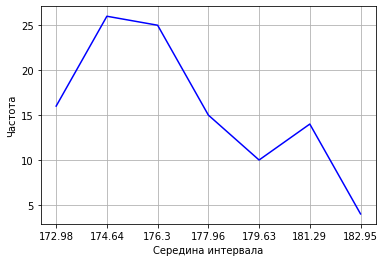
\includegraphics[width=0.9\linewidth]{male_pol_abs.png}
    \caption*{Рисунок 1 -- Полигон абсолютных частот, мужчины}
    \label{fig:1}
\end{figure}

\begin{figure}[H]
    \centering
    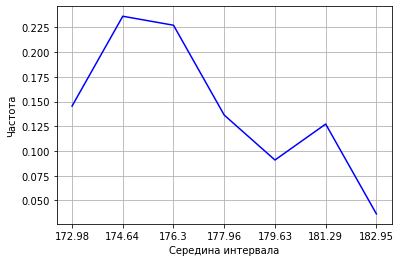
\includegraphics[width=0.9\linewidth]{male_pol_rel.png}
    \caption*{Рисунок 2 -- Полигон относительных частот, мужчины}
    \label{fig:2}
\end{figure}

\begin{figure}[H]
    \centering
    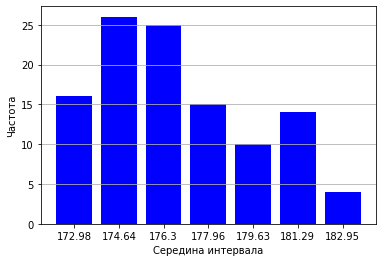
\includegraphics[width=0.9\linewidth]{male_hist_abs.png}
    \caption*{Рисунок 3 -- Гистограмма абсолютных частот, мужчины}
    \label{fig:3}
\end{figure}

\begin{figure}[H]
    \centering
    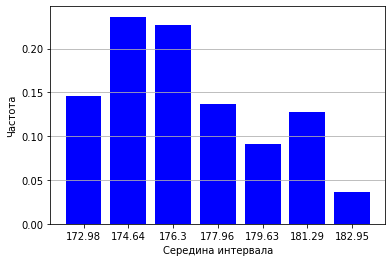
\includegraphics[width=0.9\linewidth]{male_hist_rel.png}
    \caption*{Рисунок 4 -- Гистограмма относительных частот, мужчины}
    \label{fig:4}
\end{figure}

\begin{figure}[H]
    \centering
    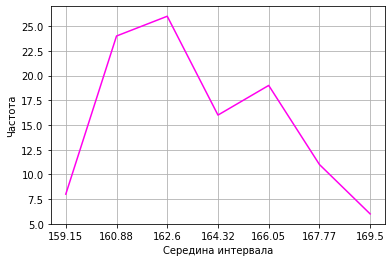
\includegraphics[width=0.9\linewidth]{female_pol_abs.png}
    \caption*{Рисунок 5 -- Полигон абсолютных частот, женщины}
    \label{fig:5}
\end{figure}

\begin{figure}[H]
    \centering
    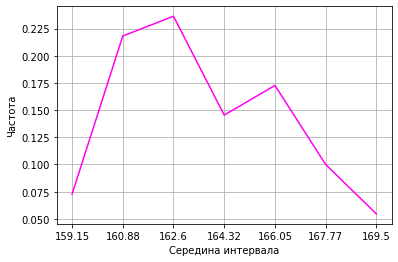
\includegraphics[width=0.9\linewidth]{female_pol_rel.png}
    \caption*{Рисунок 6 -- Полигон относительных частот, женщины}
    \label{fig:6}
\end{figure}

\begin{figure}[H]
    \centering
    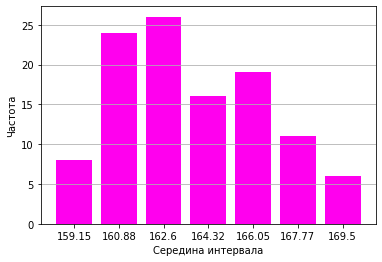
\includegraphics[width=0.9\linewidth]{female_hist_abs.png}
    \caption*{Рисунок 7 -- Гистограмма абсолютных частот, женщины}
    \label{fig:7}
\end{figure}

\begin{figure}[H]
    \centering
    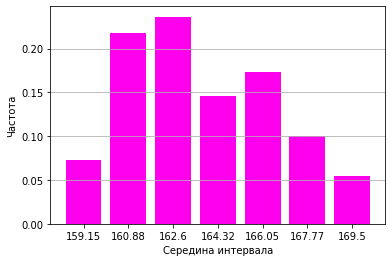
\includegraphics[width=0.9\linewidth]{female_hist_rel.png}
    \caption*{Рисунок 8 -- Гистограмма относительных частот, женщины}
    \label{fig:8}
\end{figure}

Так как выборка была ограничена 110 странами из более чем 200, и были выбраны
в среднем самые высокие, вполне ожидаемо полигоны имеют ярко выраженный <<горб>>,
но также есть дополнительный, менее выраженный горб в правом лепестке, у мужчин в районе 180 см, у женщин в районе 166.

Также построим функции распределения (см. рис. 9 и 10).

\begin{figure}[H]
    \centering
    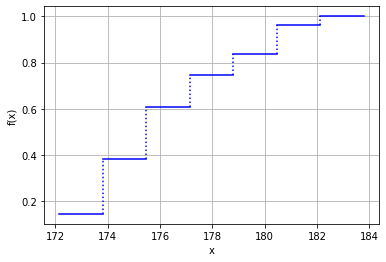
\includegraphics[width=0.9\linewidth]{male_distr.png}
    \caption*{Рисунок 9 -- Функция распределения, мужчины}
    \label{fig:9}
\end{figure}

\begin{figure}[H]
    \centering
    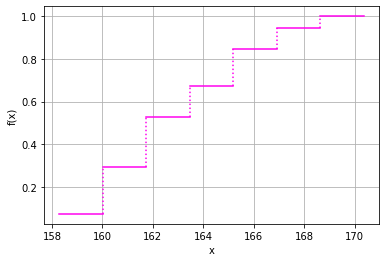
\includegraphics[width=0.9\linewidth]{female_distr.png}
    \caption*{Рисунок 10 -- Функция распределения, женщины}
    \label{fig:10}
\end{figure}

\section*{Выводы.}
В результате выполнения работы была сформирована выборка роста мужчин и женщин
в сантиметрах.
Для заданной выборки были построенные ранжированный ряд, вариационный и интервальный.
На основе интервальных рядов были построены полигоны и гистограммы абсолютных и относительных
частот.
Также были построены функции распределения.